{\textbf{{1. 路由器的工作流程}}}

\textbf{第一步:}首先路由器从线路上\textbf{接收分组},也就是下图的输入端口,经过1时进行物理层处理(进行比特的接收),经过2时进行数据链路层处理(剥去帧头、帧尾,得到了IP数据报),{然后分组就被送入网络层的模块。}

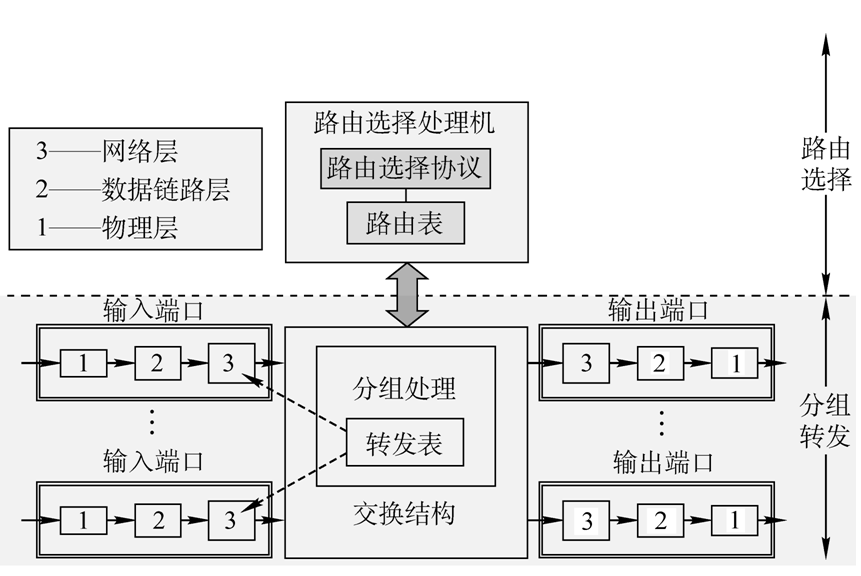
\includegraphics[width=3.12500in,height=2.09375in]{png-jpeg-pics/B52FB1366D26652412C2F046A7D7E815.png}

{\textbf{第二步:}网络层模块见下图。若接收的分组是路由器之间交换路由信息的分组(如RIP和OSPF分组),则把这种分组送交路由器的路由选择部分中的}\textbf{路由选择处理器}{。若接收的是数据分组,则按照分组首部中的目的地址查找转发表,根据得到的结果,分组就经过交换结构到达合适的输出端口。当一个分组正在查找转发表时,后面又紧跟着从这个输入端口收到另一个分组,这个分组就必须在队列中排队,因而产生了一定的时延,见下图。}

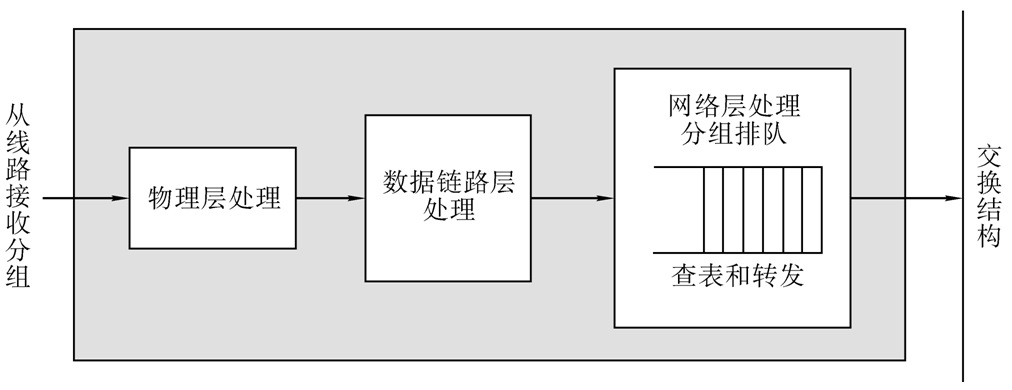
\includegraphics[width=3.22917in,height=1.23958in]{png-jpeg-pics/E3D6CF6678B98A1A530712098CF0A617.png}

\textbf{第三步:}从交换结构传送过来的分组先进行\textbf{缓存},数据链路层处理模块将给分组加上数据链路层的首部和尾部,交给\textbf{物理层}后发送到外部线路,如下图所示。

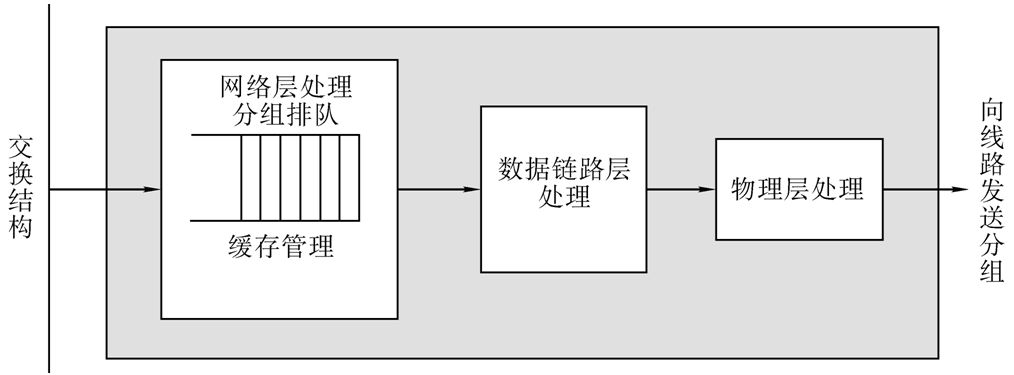
\includegraphics[width=3.33333in,height=1.22917in]{png-jpeg-pics/86F764DD73A55B076A43A7E0DAA6F103.png}
